% !TeX root = Main.tex
\chapter{Programový kód simulačního modulu}
\subsubsection*{Kód k~řešení bilineární části rovnice (\ref{rce:sim_kar_weak_real})}
Pro zápis programového kódu vztahující se k~rovnici (\ref{rce:sim_kar_weak_real}) rozdělíme bilineární část na složky reprezentované $E_{R}$ a $E_{I}$. První vyjádříme zápis, který je v~programu označen indexem \uv{real\_real}. Rozepsáním operátoru $\nabla$ a numerickým řešením integrálů obdržíme výraz
\begin{equation}
	-\sum_{i=0}^{n}\mathrm{w}_{t}[i]\bigg(\frac{\partial E_R}{\partial x}\cdot \frac{\partial v}{\partial x} + \frac{\partial E_R}{\partial y}\cdot \frac{\partial v}{\partial y} \bigg) + \omega^{2}\varepsilon\mu\sum_{i=0}^{n}\mathrm{w}_{t}[i]\bigg(E_R\cdot v\bigg),
	\label{rce:sim_kar_weak_real_real_num} 
\end{equation}
Vlastní programový kód, který implemetuje bilineární část (\ref{rce:sim_kar_weak_real_real_num}), je následující

\begin{verbatim}
template<typename Real, typename Scalar>
Scalar rf_matrix_form_real_real(int n, double *wt, Func<Real> *u_ext[], Func<Real> *u,
                                    Func<Real> *v, Geom<Real> *e, ExtData<Scalar> *ext)
{
    return - int_grad_u_grad_v<Real, Scalar>(n, wt, u, v)
    + sqr(2 * M_PI * frequency) * (rfLabel[e->elem_marker].permeability * MU0)
    * (rfLabel[e->elem_marker].permittivity * EPS0) * int_u_v<Real, Scalar>(n, wt, u, v);
}
\end{verbatim}
Obdobným způsobem postupujeme u~druhé složky bilineární části vyjádřené pomocí $E_I$. Index funkce v~programu se změní na \uv{real\_imag}
\begin{equation}
 \omega\mu\sigma\sum_{i=0}^{n}\mathrm{w}_{t}[i]\bigg(E_I\cdot v\bigg)
	\label{rce:sim_kar_weak_real_imag_num} 
\end{equation}
Vztah \ref{rce:sim_kar_weak_real_imag_num} se analogicky zapíše jako
\begin{verbatim}
template<typename Real, typename Scalar>
Scalar rf_matrix_form_real_imag(int n, double *wt, Func<Real> *u_ext[], Func<Real> *u,
                                     Func<Real> *v, Geom<Real> *e, ExtData<Scalar> *ext)
{
    return + 2 * M_PI * frequency * (rfLabel[e->elem_marker].permeability * MU0) 
    * rfLabel[e->elem_marker].conductivity * int_u_v<Real, Scalar>(n, wt, u, v);
}
\end{verbatim}

\subsubsection*{Kód k~řešení bilineární části rovnice (\ref{rce:sim_kar_weak_imag})}
Postup je naprosto totožný jako u~slabé formy reálné složky výchozí rovnice. Tudíž opět rozdělíme bilineární část na 2 části dle $E_R$ a $E_I$. Dále zavedeme numerickou integraci a zapíšeme vzniklé výrazy do programového kódu. Pro index \uv{imag\_real} platí
\begin{equation}
 -\omega\mu\sigma\sum_{i=0}^{n}\mathrm{w}_{t}[i]\bigg(E_I\cdot v\bigg)
	\label{rce:sim_kar_weak_imag_real_num} 
\end{equation}
\begin{verbatim}
template<typename Real, typename Scalar>
Scalar rf_matrix_form_imag_real(int n, double *wt, Func<Real> *u_ext[], Func<Real> *u,
									Func<Real> *v, Geom<Real> *e, ExtData<Scalar> *ext)
{
    return - 2 * M_PI * frequency * (rfLabel[e->elem_marker].permeability * MU0) 
    * rfLabel[e->elem_marker].conductivity * int_u_v<Real, Scalar>(n, wt, u, v);
}
\end{verbatim}
Nakonec pro označení \uv{imag\_imag}
\begin{equation}
	-\sum_{i=0}^{n}\mathrm{w}_{t}[i]\bigg(\frac{\partial E_I}{\partial x}\cdot \frac{\partial v}{\partial x} + \frac{\partial E_I}{\partial y}\cdot \frac{\partial v}{\partial y} \bigg) + \omega^{2}\varepsilon\mu\sum_{i=0}^{n}\mathrm{w}_{t}[i]\bigg(E_I\cdot v\bigg),
	\label{rce:sim_kar_weak_imag_imag_num} 
\end{equation}
\begin{verbatim}
template<typename Real, typename Scalar>
Scalar rf_matrix_form_imag_imag(int n, double *wt, Func<Real> *u_ext[], Func<Real> *u,
                                    Func<Real> *v, Geom<Real> *e, ExtData<Scalar> *ext)
{
    return - int_grad_u_grad_v<Real, Scalar>(n, wt, u, v) 
    + sqr(2 * M_PI * frequency) * (rfLabel[e->elem_marker].permeability * MU0) 
    * (rfLabel[e->elem_marker].permittivity * EPS0) * int_u_v<Real, Scalar>(n, wt, u, v);
}
\end{verbatim}

\subsubsection*{Zápis lineárních členů rovnic (\ref{rce:sim_kar_weak_real}) a (\ref{rce:sim_kar_weak_imag}).}
Lineární členy jsou vyjádřeny jako pravé strany rovnic (\ref{rce:sim_kar_weak_real}) a (\ref{rce:sim_kar_weak_imag}). Jsou tudíž nulové, ale pro vlastní numerické řešení je potřeba tuto informaci doplnit do programového kódu. Vzhledem k~tomu, že řešená rovnice je komplexního charakteru je potřeba doplnit tyto dvě funkce 

\begin{verbatim}
template<typename Real, typename Scalar>
Scalar rf_vector_form_real(int n, double *wt, Func<Real> *u_ext[], Func<Real> *v,
                                               Geom<Real> *e, ExtData<Scalar> *ext)
{
    return 0.0;
}
\end{verbatim}
\begin{verbatim}
template<typename Real, typename Scalar>
Scalar rf_vector_form_imag(int n, double *wt, Func<Real> *u_ext[], Func<Real> *v, 
                                              Geom<Real> *e, ExtData<Scalar> *ext)
{
    return 0.0;
}
\end{verbatim}
Zmíněné funkce pro řešení Helmholtzovy rovnice (\ref{rce:sim_kar_helmholtz_num}) je dále potřeba zaregistrovat ve třídě \textsc{WeakForm} následujícím způsobem
\begin{verbatim}
wf->add_matrix_form(0, 0, callback(rf_matrix_form_real_real));
wf->add_matrix_form(0, 1, callback(rf_matrix_form_real_imag));
wf->add_matrix_form(1, 0, callback(rf_matrix_form_imag_real));
wf->add_matrix_form(1, 1, callback(rf_matrix_form_imag_imag));
wf->add_vector_form(0, callback(rf_vector_form_real))
wf->add_vector_form(1, callback(rf_vector_form_imag));
\end{verbatim}

\subsubsection*{Numerické řešení rovnice (\ref{rce:sim_pol_helmholtz_upravena})}
Bilineární člen dané slabé formy s~indexem \uv{real\_real} lze po zavedení numerické integrace zapsat jako
\begin{displaymath}
-\sum_{i=0}^{n}\mathrm{w}_{t}[i]\bigg(\frac{\partial E_{\alpha R}}{\partial z}\cdot \frac{\partial v}{\partial z} + \frac{\partial E_{\alpha R}}{\partial r}\cdot \frac{\partial v}{\partial r} \bigg) - \frac{1}{r}\sum_{i=0}^{n}\mathrm{w}_{t}[i]\bigg(\frac{\partial E_{\alpha R}}{\partial r}\cdot v\bigg) +
\end{displaymath}
\begin{equation}
	 + \frac{1}{r^{2}}\sum_{i=0}^{n}\mathrm{w}_{t}[i]\bigg(E_{\alpha R}\cdot v\bigg) + \omega^{2}\varepsilon\mu\sum_{i=0}^{n}\mathrm{w}_{t}[i]\bigg(E_{\alpha R}\cdot v\bigg).
	\label{rce:sim_pol_bilinear_real_real} 
\end{equation}
Je zřejmé, že forma označená \uv{real\_imag} vyjde identicky jako v~případě kartézské souřadné soustavy, neboť člen $+\faz k^{2}\faz E_{\alpha}$ v~rovnici (\ref{rce:sim_pol_helmholtz_upravena}) je formálně stejný se vztahem (\ref{rce:sim_kar_helmholtz_num}). Platí tedy
\begin{equation}
 \omega\mu\sigma\sum_{i=0}^{n}\mathrm{w}_{t}[i]\bigg(E_{\alpha I}\cdot v\bigg).
	\label{rce:sim_pol_bilinear_real_imag} 
\end{equation}
Slabým formám vycházející z~imaginární části z~původní rovnice (\ref{rce:sim_pol_helmholtz_upravena}) odpovídá vyjádření
\begin{equation}
 -\omega\mu\sigma\sum_{i=0}^{n}\mathrm{w}_{t}[i]\bigg(E_{\alpha R}\cdot v\bigg)
	\label{rce:sim_pol_bilinear_imag_imag} 
\end{equation}
pro \uv{imag\_real}, což je opět ze stejného důvodu identické s~kartézskou souřadnou soustvou. Nakonec indexu \uv{imag\_imag} odpovídá
\begin{displaymath}
-\sum_{i=0}^{n}\mathrm{w}_{t}[i]\bigg(\frac{\partial E_{\alpha I}}{\partial z}\cdot \frac{\partial v}{\partial z} + \frac{\partial E_{\alpha I}}{\partial r}\cdot \frac{\partial v}{\partial r} \bigg) - \frac{1}{r}\sum_{i=0}^{n}\mathrm{w}_{t}[i]\bigg(\frac{\partial E_{\alpha I}}{\partial r}\cdot v\bigg) +
\end{displaymath}
\begin{equation}
	 + \frac{1}{r^{2}}\sum_{i=0}^{n}\mathrm{w}_{t}[i]\bigg(E_{\alpha I}\cdot v\bigg) + \omega^{2}\varepsilon\mu\sum_{i=0}^{n}\mathrm{w}_{t}[i]\bigg(E_{\alpha I}\cdot v\bigg).
	\label{rce:sim_pol_bilinear_real_real} 
\end{equation}
Vzhledem k~nulové pravé straně řešené výchozí rovnice (\ref{rce:sim_pol_helmholtz_upravena}) bude lineární člen  v~tomto případě opět nulový.





\section{Vlastnosti prostředí}
V~řešené rovnici (\ref{rce:sim_kar_helmholtz_num}) vystupují také materiálové konstatny prostředí, ve kterém se elektromagnetická vlna šíří. Pro jejich specifikaci je potřeba vytvořit materiál s~těmito konstantami a vhodně jej přiřadit k~příslušným značkám oblastí. Zpřístupnit dialog pro výběr lze opět pravým kliknutím na pracovní plochu a vybráním možnosti \uv{new material}, eventuelně zkratkou Alt + M. 
\begin{figure}[!h]
	\centering
	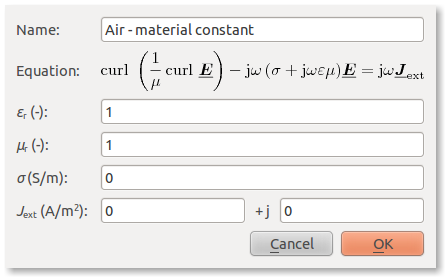
\includegraphics[width=7cm]{sim_material.png}
	\caption{Vytvoření materiálu vzduchu zadáním konstant prostředí.}
	\label{obr:sim_material}
\end{figure}
Parametry $\varepsilon_r$ a $\mu_r$ představují, tak jak je běžně používané, relativní hodnoty permitivity a permeability. Pomocí $\sigma$ zadáme vodivost v~daném prostředí. Poslední parametr $J_{ext}$ představuje vnucený proud do oblasti, která je reprezentovaná danou značkou.

Programová implementace $J_{ext}$ spočívá v~řešení Helmholtzovy rovnice (\ref{rce:sim_kar_helmholtz_num}) v~případě nenulové pravé strany. Ta po převedení rovnice na slabou formu představuje její lineární část a je tak potřeba s~ní nakládat. Vstupní rovnice pro implemetaci vnucené proudové hustoty je tedy
\begin{displaymath}
	\nabla^{2}\vecfaz E +\faz k^{2}\vecfaz E = \mathrm{grad}\frac{\rho}{\varepsilon} + \mj\omega\mu J_{ext}.
\end{displaymath}
Člen $\mathrm{grad}\frac{\rho}{\varepsilon}$ je možné zanedbat, vzhledem k~předpokladu rovnoměrného rozložení náboje $\rho$. Při této úvaze bude hodnota gradientu nulová. Při převodu na slabou formu vyjádříme samostatně reálnou a imaginární složku vnější proudové husototy.
\begin{displaymath}
	\nabla^{2}(E_R + \mj E_I) + (\omega^{2}\varepsilon\mu - \mj\omega\mu\sigma)(E_R + \mj E_I) = \mj\omega\mu (J_{ext R} + \mj J_{ext I}). 
\end{displaymath}
Po rozdělení a převodu na slabé formy stejným způsobem jako v~podkapitole \ref{sec:sim_hermes2d} dostaneme vztahy, ve kterých na pravé straně vystupují lineární členy 
\begin{equation}
	\Re : -\int_{\Omega}\nabla E_R\cdot\nabla v~\dif S~+ \omega^{2}\varepsilon\mu\int_{\Omega} E_R\cdot v\dif S~+ \omega\mu\sigma\int_{\Omega} E_I\cdot v\dif S~= -\omega\mu J_{ext I},
	\label{rce:sim_jext_real} 
\end{equation}
\begin{equation}
	\Im : -\int_{\Omega}\nabla E_I\cdot\nabla v\dif S~+ \omega^{2}\varepsilon\mu\int_{\Omega} E_I\cdot v\dif S~- \omega\mu\sigma\int_{\Omega} E_R\cdot v\dif S~= \omega\mu J_{ext R}.
	\label{rce:sim_jext_imag} 
\end{equation}










\subsection{Okrajové podmínky v~simulačním modulu}
Při řešení problémů vztahující se k~elektromagnetickému poli je možné použít na řešenou oblast několik typů okrajových podmínek, které se zadávají v~dialogu \uv{new boundary condition}. Ten je možné zpřístupnit po pravém kliknutí na pracovní plochu a vybrání daného odkazu, případně je možné se na něj dostat klávesovou zkratkou Alt + B. Po zadání označení se vybere v~rozbalovacím menu některá z~definovaných okrajových podmínek.

\subsubsection*{Electric field}
První možností je zadat Dirichletovu podmínka na určité hranici $\Gamma$. Hodnotu okrajové podmínky zadáme jako komplexní číslo ve formátu reálné a imaginární složky, jak je znázorněno na obrázku \ref{obr:sim_BC_electric_field} pro číslo $0 + \mj 0$. Tato konkrétní okrajová podmínka se v~oboru vysokofrekvenční techniky označuje jako \uv{perfect electric conductor}.
\begin{figure}[!h]
	\centering
	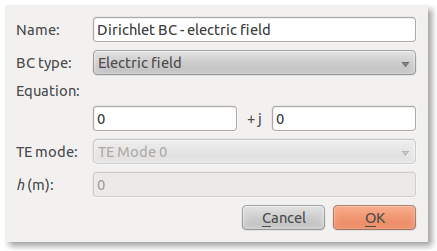
\includegraphics[width=7cm]{sim_BC_electric_field.png}
	\caption{Zadání Dirichletovy podmínky $0 + \mj 0$ pro elektrickou složku pole.}
	\label{obr:sim_BC_electric_field}
\end{figure}

Programový kód, který přísluší k~této okrajové podmínce, je v~modulu zapsán nastavením tříd \textsc{BCTypes} a \textsc{BCValues} následovně
\begin{verbatim}
BCTypes bcTypesReal, bcTypesImag;
bcTypesReal.add_bc_dirichlet(i+1);
bcTypesImag.add_bc_dirichlet(i+1);
                
BCValues bcValuesReal, bcValuesImag;
bcValuesReal.add_const(i+1, edgeRFMarker->value_real.number);
bcValuesImag.add_const(i+1, edgeRFMarker->value_imag.number);
\end{verbatim}

\subsubsection*{Magnetic field}
Touto volbou zadáváme hodnotu normálové derivace funkce $\frac{\partial E_{(z)}}{\partial n}$, jenž představuje Neumannovu okrajovou podmínku na hranici $\Gamma$. Opět má charakter komplexní veličiny, ve slabých formách vyjádřených v~(\ref{rce:sim_kar_weak_real} ) a (\ref{rce:sim_kar_weak_imag}) podmínka představuje členy $\int_{\Gamma}\frac{\partial E_R}{\partial n}\cdot v\dif l$, případně $\int_{\Gamma}\frac{\partial E_I}{\partial n}\cdot v\dif l$. Příslušný kód je zapsán třídou \textsc{BCTypes}
\begin{verbatim}
BCTypes bcTypesReal, bcTypesImag;
bcTypesReal.add_bc_neumann(i+1);
bcTypesImag.add_bc_neumann(i+1);               
\end{verbatim}
a funkcí vracející povrchovou lineární formu Neumannovy okrajové podmínky. V~případě nulové Neumannovy okrajové podmínky však lze danou funkci vynechat, tak jako v~tomto případě.

\subsubsection*{Matched boundary}
Pokud chceme na určené hranici zvolit impedanční přizpůsobení, učiníme tak v~dialogu pro výběr následující možností dle obrázku \ref{obr:sim_BC_matched_boundary}. 
\begin{figure}[!h]
	\centering
	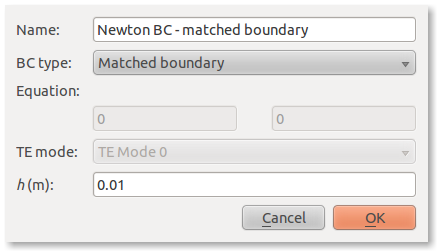
\includegraphics[width=7cm]{sim_BC_matched_boundary.png}
	\caption{Zadání impedančního přizpůsobení.}
	\label{obr:sim_BC_matched_boundary}
\end{figure}
Je zde možné zadat výšku hranice na kterou chceme aplikovat impedanční přizpůsobení pro výpočet konstatny $\beta$ ve vztahu (\ref{rce:sim_BC_matched_boundary}). V~případě, že výšku nezadáme, bude výpočet impedančního přizpůsobení vycházet z~vlnové impedance prostředí $Z = \frac{\omega\mu}{\beta}$. Ve výpočtu se tedy jedná se o~Newtonovu okrajovou podmínku ve tvaru
\begin{equation}
	\bigg(\frac{\partial E_{(z)}}{\partial n} - \mj\beta E_{(z)}\bigg)|_{\Gamma} = 0.
	\label{rce:sim_BC_matched_boundary}
\end{equation}
Pro její implementaci je potřeba nastavit třídu \textsc{BCTypes} následovně
\begin{verbatim}
BCTypes bcTypesReal, bcTypesImag;
bcTypesReal.add_bc_newton(i+1);
bcTypesImag.add_bc_newton(i+1);              
\end{verbatim}
a také zapsat funkce pro povrchové bilineární formy. Pro reálnou složku odpovídá 
\begin{verbatim}
template<typename Real, typename Scalar>
Scalar rf_matrix_form_surf_imag_real(int n, double *wt, Func<Real> *u_ext[], Func<Real> *u,
                                         Func<Real> *v, Geom<Real> *e, ExtData<Scalar> *ext)
{
    if (!(rfEdge[e->edge_marker].type == PhysicFieldBC_RF_MatchedBoundary ||
          rfEdge[e->edge_marker].type == PhysicFieldBC_RF_Port))
    return 0.0;

    double mu = rfLabel[e->elem_marker].permeability * MU0;
    double eps = rfLabel[e->elem_marker].permittivity * EPS0;
    double height = rfEdge[e->edge_marker].height;
    double beta = 0.0;
    double Z~= 0.0;

    if(!rfEdge[e->edge_marker].height == 0)
    {
        beta = sqrt(sqr(2 * M_PI * frequency) * mu * eps - sqr(1 * M_PI / height));
        return beta * int_u_v<Real, Scalar>(n, wt, u, v);
    }
    else
    {
        beta = sqrt(sqr(2 * M_PI * frequency) * mu * eps);
        Z~= ((2 * M_PI * frequency) * mu ) / beta;
        return Z~* int_u_v<Real, Scalar>(n, wt, u, v);
    }
}
\end{verbatim}
Pro imaginární část okrajové podmínky platí
\begin{verbatim}
template<typename Real, typename Scalar>
Scalar rf_matrix_form_surf_real_imag(int n, double *wt, Func<Real> *u_ext[], Func<Real> *u,
                                         Func<Real> *v, Geom<Real> *e, ExtData<Scalar> *ext)
{
    if (!(rfEdge[e->edge_marker].type == PhysicFieldBC_RF_MatchedBoundary ||
          rfEdge[e->edge_marker].type == PhysicFieldBC_RF_Port))
    return 0.0;

    double mu = rfLabel[e->elem_marker].permeability * MU0;
    double eps = rfLabel[e->elem_marker].permittivity * EPS0;
    double height = rfEdge[e->edge_marker].height;
    double beta = 0.0;
    double Z~= 0.0;

    if(!rfEdge[e->edge_marker].height == 0)
    {
        beta = sqrt(sqr(2 * M_PI * frequency) * mu * eps - sqr(1 * M_PI / height));
        return beta * int_u_v<Real, Scalar>(n, wt, u, v);
    }
    else
    {
        beta = sqrt(sqr(2 * M_PI * frequency) * mu * eps);
        Z~= ((2 * M_PI * frequency) * mu ) / beta;
        return Z~* int_u_v<Real, Scalar>(n, wt, u, v);
    }
}
\end{verbatim}
Lineární část je u~vztahu (\ref{rce:sim_BC_matched_boundary}) nulová, proto lze funkci pro její zápis vynechat.
Nakonec je potřeba výše uvedené funkce zaregistrovat ve třídě \textsc{WeakForm} takto
\begin{verbatim}
wf->add_vector_form_surf(0, callback(rf_vector_form_surf_real));
wf->add_vector_form_surf(1, callback(rf_vector_form_surf_imag));           
\end{verbatim}
                
\subsubsection*{Port}

\section{Možnosti zobrazení výsledků řešení}
Vlastnosti postprocessingu zobrazení v~programu Agors2D jsou velmi obsáhlé. Pomocí levého panelu v~pracovním okně (patrné na obrázku \ref{obr:sim_agros2d}) je možné vybrat zobrazení ve 2D nebo 3D prostoru. Dále je možno aktivovat nebo skrýt geometrii,  diskretizační síť, kontury zobrazení a také odpovídající vektory. V~bloku týkající se skalárního pole lze vybrat zobrazení požadovaných veličin, které se týkají řešení daného fyzikálního pole. Příslušné vztahy pro interpretaci výsledků je však potřeba implemetovat v~samostatném modulu, patřící k~jednotlivým polím.

\subsection{Vztahy pro zobrazení veličin elektromagnetického pole}
V~případě elektromagnetického pole nás bude zajímat především rozložení elektrického a magnetického pole, magnetické indukce, Poyntingova vektoru a ztrát. Zobrazení těchto  veličin a jejich odpovídajících složek lze vybrat z~rozbalovacího menu, které je patrné na obrázku \ref{obr:sim_zobrazeni}.
\begin{figure}[!h]
	\centering
	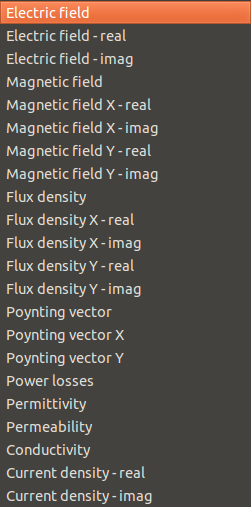
\includegraphics[width=4cm]{sim_zobrazeni.png}
	\caption{Volba veličiny pro zobrazení.}
	\label{obr:sim_zobrazeni}
\end{figure}
 
\subsection*{Electric field}
Programová implementace pro elektrickou složku pole v~kartézských souřanicích je v~modulu zajištěn ve funkci \texttt{ViewScalarFilterRF} pomocí následujícího kódu
\begin{verbatim}
node->values[0][0][i] = sqrt(sqr(value1[i]) + sqr(value2[i]));
\end{verbatim}
kde je patrná reálná složka elektrického pole, jejíž samostatný zápis v~modulu je
\begin{verbatim}
node->values[0][0][i] = value1[i];
\end{verbatim}
a obdobně imaginární složka 
\begin{verbatim}
node->values[0][0][i] = value2[i];
\end{verbatim}

\subsection*{Magnetic flux density}
Odvození vztahů pro zobrazení magnetické indukce vychází z~druhého Maxwellova zákona (\ref{rce:1MaxwR}), který má pro harmonické pole tvar
\begin{displaymath}
	rot\vec E = -\mj\omega\vec B.
\end{displaymath}
Po úpravě rotace na levé straně výrazu pro jedinou složku $E_z$ dostaneme vztah
\begin{equation}
	\frac{\partial E_z}{\partial y}\cdot\overrightarrow{\vec{i}} - \frac{\partial E_z}{\partial y}\cdot\overrightarrow{\vec{j}} + 0\cdot\overrightarrow{\vec{k}} = -\mj\omega B_x\cdot\overrightarrow{\vec{i}} - \mj\omega B_y\cdot\overrightarrow{\vec{j}} - \mj\omega B_z\cdot\overrightarrow{\vec{k}},
	\label{rce:sim_zobrazeni_flux}
\end{equation}
ze kterého lze vyjádřit $x$-ová a $y$-ová složka magnetické indukce. $B_z$ je podle rovnice (\ref{rce:sim_zobrazeni_flux}) nulová. Pro $B_x$ tedy platí
\begin{displaymath}
	B_x = -\frac{1}{\mj\omega}\frac{\partial E_z}{\partial y},
\end{displaymath}
kde po dosazení za $E_z$ můžeme vyjádřit reálnou a imaginární složku magnetické indukce ve směru x a ty pak implemetovat do modulu. Reálné části odpovídá 
\begin{equation}
	B_{x\Re} = -\frac{1}{\mj\omega}\frac{\partial E_I}{\partial y},
	\label{rce:sim_flux_x_re}
\end{equation}
a její programový kód ve funkci \texttt{ViewScalarFilterRF}
\begin{verbatim}
case PhysicFieldVariable_RF_MagneticFluxDensityXReal:
{
    double w = 2 * M_PI * Util::scene()->problemInfo()->frequency;
    node->values[0][0][i] = -(1/(w)) * dudy2[i];
}
\end{verbatim}
Analogickým způsobem platí pro imaginární část
\begin{equation}
	B_{x\Im} = \frac{1}{\mj\omega}\frac{\partial E_R}{\partial y}.
	\label{rce:sim_flux_x_im}
\end{equation}
\begin{verbatim}
case PhysicFieldVariable_RF_MagneticFluxDensityXImag:
{
    double w = 2 * M_PI * Util::scene()->problemInfo()->frequency;
    node->values[0][0][i] = (1/(w)) * dudy1[i];
}    
\end{verbatim}
Z~rovnice (\ref{rce:sim_zobrazeni_flux}) je pak dále možné stejným způsobem odvodit vztahy pro obě složky indukce ve směru $y$, která je označná $B_y$, včetně její implementace
\begin{equation}
	B_{y\Re} = \frac{1}{\mj\omega}\frac{\partial E_I}{\partial x},
	\label{rce:sim_flux_y_re}
\end{equation}
\begin{verbatim}
case PhysicFieldVariable_RF_MagneticFluxDensityYReal:
{
    double w = 2 * M_PI * Util::scene()->problemInfo()->frequency;
    node->values[0][0][i] = (1/(w)) * dudx2[i];
}
\end{verbatim}
\begin{equation}
	B_{y\Im} = -\frac{1}{\mj\omega}\frac{\partial E_R}{\partial x},
	\label{rce:sim_flux_y_im}
\end{equation}
\begin{verbatim}
case PhysicFieldVariable_RF_MagneticFluxDensityYImag:
{
    double w = 2 * M_PI * Util::scene()->problemInfo()->frequency;
    node->values[0][0][i] = -(1/(w)) * dudx1[i];
}
\end{verbatim}
Nakonec zbývá vyjádřit rozložení vektoru magnetické indukce. Pro jeho velikost platí
\begin{displaymath}
	B = \sqrt{B_{x}^{2} + B_{y}^{2}} = \sqrt{B_{x\Re}^{2} + B_{x\Im}^{2} + B_{y\Re}^{2} + B_{y\Im}^{2}}
\end{displaymath}
což je možné v~programovém kódu zapsat takto
\begin{verbatim}
case PhysicFieldVariable_RF_MagneticFluxDensity:
{
    double w = 2 * M_PI * Util::scene()->problemInfo()->frequency;
    node->values[0][0][i] = sqrt(sqr(-(1/(w)) * dudy2[i]) + sqr((1/(w)) * dudy1[i])
                               + sqr((1/(w)) * dudx2[i]) + sqr(-(1/(w)) * dudx1[i]));
}
\end{verbatim}

\subsection*{Magnetic field}
Vztahy pro zobrazení magnetického pole s~výhodou vycházejí z~již vyjádřené magnetické indukce, neboť platí
\begin{displaymath}
H = \frac{1}{\mu}\cdot B.
\end{displaymath}
Je zřejmé, že veškeré výše odvozené vztahy (\ref{rce:sim_flux_x_re}) až (\ref{rce:sim_flux_y_im}) lze pouze podělit hodnotou permeability, která se v~nachází na řešené oblasti. Pro úplnost je níže uveden kód pro reálnou složku intenzity magnetického pole ve směru $x$, tj. $H_{x\Re}$
\begin{verbatim}
case PhysicFieldVariable_RF_MagneticFieldXReal:
{
    SceneMaterialRF *marker = dynamic_cast<SceneMaterialRF *>(material);
    double mu = marker->permeability.number * MU0;
    double w = 2 * M_PI * Util::scene()->problemInfo()->frequency;
    node->values[0][0][i] = -(1/(w*mu)) * dudy2[i];
}
\end{verbatim}

\subsection*{Poyntingův vektor}
Vektor vyjádřený vektorovým součinem intenzit elektrického a magnetického pole představuje plošnou hustotu výkonu na řešené oblasti $\Omega$
\begin{displaymath}
	\vec N = \vec E \times\vec H.
\end{displaymath}
Programový kód pro rozložení Poyntingova vektoru ve směru $x$ vychází ze vztahu
\begin{displaymath}
	N_x = \frac{E_I H_{y\Im} + E_R H_{y\Re}}{2}
\end{displaymath}
je v~modulu zapsán takto
\begin{verbatim}
case PhysicFieldVariable_RF_PoyntingVectorX:
{
    SceneMaterialRF *marker = dynamic_cast<SceneMaterialRF *>(material);
    double mu = marker->permeability.number * MU0;
    double w = 2 * M_PI * Util::scene()->problemInfo()->frequency;
    node->values[0][0][i] = - 0.5 * ((value2[i] * 1/(w*mu) * dudx1[i]) - (value1[i] * 1/(w*mu) * dudx2[i]));
}
\end{verbatim}
Pro Poyntingův vektor ve směru $y$ analogicky platí
\begin{displaymath}
	N_y = \frac{E_I H_{x\Im} + E_R H_{x\Re}}{2}
\end{displaymath}
\begin{verbatim}
case PhysicFieldVariable_RF_PoyntingVectorY:
{
    SceneMaterialRF *marker = dynamic_cast<SceneMaterialRF *>(material);
    double mu = marker->permeability.number * MU0;
    double w = 2 * M_PI * Util::scene()->problemInfo()->frequency;
    node->values[0][0][i] = 0.5 * ((value2[i] * 1/(w*mu) * dudy1[i]) - (value1[i] * 1/(w*mu) * dudy2[i]));
}
\end{verbatim}
Pro výslednou hodnotu Poyntingova vektoru na řešené oblasti $\Omega$ platí
\begin{displaymath}
	N = \sqrt{N_{x}^{2} + N_{y}^{2}} = \frac{1}{2}\cdot\sqrt{(E_I H_{y\Im} + E_R H_{y\Re})^{2} + (E_I H_{x\Im} + E_R H_{x\Re})^{2}}.
\end{displaymath}
\begin{verbatim}
case PhysicFieldVariable_RF_PoyntingVector:
{
    double mu = marker->permeability.number * MU0;
    double w = 2 * M_PI * Util::scene()->problemInfo()->frequency;
    node->values[0][0][i] = 0.5 * sqrt(sqr(((value2[i] * 1/(w*mu) * dudx1[i]) 
                                          - (value1[i] * 1/(w*mu) * dudx2[i]))) 
                                     + sqr(((value2[i] * 1/(w*mu) * dudy1[i]) 
                                          - (value1[i] * 1/(w*mu) * dudy2[i]))));
}
\end{verbatim}

\subsection*{Ztráty}
Rozložení ztrát v~řešené oblasti odpovídá součinu proudové husoty a intenzity elektrického pole 
\begin{displaymath}
	P_j = J \cdot E = \sigma E^{2} = \sigma \sqrt{E_{R}^{2} + E_{I}^{2}}.
\end{displaymath}
Zápis kódu má následující charakter
\begin{verbatim}
case PhysicFieldVariable_RF_PowerLosses:
{
    double sigma = (marker->conductivity.number);
    node->values[0][0][i] = 0.5 * (sqr(value1[i]) + sqr(value2[i])) * sigma;
}
\end{verbatim}


% !TeX root = Main.tex
\chapter{Programový kód simulačního modulu} \label{kap:Program_kod}
\section{Řešení Helmholtzovy rovnice (\ref{rce:sim_kar_helmholtz_num}) knihovnou Hermes2D}
\subsubsection*{Reálná část (\ref{rce:sim_kar_weak_real})}
Implementace bilineární části odpovídá následujícím zápisům
\begin{verbatim}
template<typename Real, typename Scalar>
Scalar rf_matrix_form_real_real(int n, double *wt, Func<Real> *u_ext[], Func<Real> *u,
                                    Func<Real> *v, Geom<Real> *e, ExtData<Scalar> *ext)
{
    return - int_grad_u_grad_v<Real, Scalar>(n, wt, u, v)
    + sqr(2 * M_PI * frequency) * (rfLabel[e->elem_marker].permeability * MU0)
    * (rfLabel[e->elem_marker].permittivity * EPS0) * int_u_v<Real, Scalar>(n, wt, u, v);
}

template<typename Real, typename Scalar>
Scalar rf_matrix_form_real_imag(int n, double *wt, Func<Real> *u_ext[], Func<Real> *u,
                                     Func<Real> *v, Geom<Real> *e, ExtData<Scalar> *ext)
{
    return + 2 * M_PI * frequency * (rfLabel[e->elem_marker].permeability * MU0) 
    * rfLabel[e->elem_marker].conductivity * int_u_v<Real, Scalar>(n, wt, u, v);
}

\end{verbatim}
Lineární člen na pravé straně rovnice je potřeba zapsat ve tvaru
\begin{verbatim}
template<typename Real, typename Scalar>
Scalar rf_vector_form_real(int n, double *wt, Func<Real> *u_ext[], Func<Real> *v,
                                              Geom<Real> *e, ExtData<Scalar> *ext)
{
    Scalar result = 0 ;
    int u = 0;
    for (int i = 0; i < n; i++)
        result += wt[i] * (rfLabel[e->elem_marker].current_density_imag * v->val[i]);

    return - 2 * M_PI * frequency * (rfLabel[e->elem_marker].permeability * MU0) * result;
}
\end{verbatim}

\subsubsection*{Imaginární část (\ref{rce:sim_kar_weak_imag})}
Složky kódu s~indexy \uv{imag\_real} a \uv{imag\_imag} jsou zapsána
\begin{verbatim}
template<typename Real, typename Scalar>
Scalar rf_matrix_form_imag_real(int n, double *wt, Func<Real> *u_ext[], Func<Real> *u,
									Func<Real> *v, Geom<Real> *e, ExtData<Scalar> *ext)
{
    return - 2 * M_PI * frequency * (rfLabel[e->elem_marker].permeability * MU0) 
    * rfLabel[e->elem_marker].conductivity * int_u_v<Real, Scalar>(n, wt, u, v);
}

template<typename Real, typename Scalar>
Scalar rf_matrix_form_imag_imag(int n, double *wt, Func<Real> *u_ext[], Func<Real> *u,
                                    Func<Real> *v, Geom<Real> *e, ExtData<Scalar> *ext)
{
    return - int_grad_u_grad_v<Real, Scalar>(n, wt, u, v) 
    + sqr(2 * M_PI * frequency) * (rfLabel[e->elem_marker].permeability * MU0) 
    * (rfLabel[e->elem_marker].permittivity * EPS0) * int_u_v<Real, Scalar>(n, wt, u, v);
}
\end{verbatim}
Nakonec lineární člen imaginární části řešené rovnice je implemetován zápisem
\begin{verbatim}
template<typename Real, typename Scalar>
Scalar rf_vector_form_imag(int n, double *wt, Func<Real> *u_ext[], Func<Real> *v,
                                              Geom<Real> *e, ExtData<Scalar> *ext)
{
    Scalar result = 0 ;
    int u~= 0;
    for (int i = 0; i < n; i++)
        result += wt[i] * (rfLabel[e->elem_marker].current_density_real * v->val[i]);

    return 2 * M_PI * frequency * (rfLabel[e->elem_marker].permeability * MU0) * result;
}
\end{verbatim}
\subsubsection*{Registrace forem}
Zmíněné funkce pro řešení Helmholtzovy rovnice (\ref{rce:sim_kar_helmholtz_num}) je dále potřeba zaregistrovat ve třídě \textsc{WeakForm} následujícím způsobem
\begin{verbatim}
wf->add_matrix_form(0, 0, callback(rf_matrix_form_real_real));
wf->add_matrix_form(0, 1, callback(rf_matrix_form_real_imag));
wf->add_matrix_form(1, 0, callback(rf_matrix_form_imag_real));
wf->add_matrix_form(1, 1, callback(rf_matrix_form_imag_imag));
wf->add_vector_form(0, callback(rf_vector_form_real))
wf->add_vector_form(1, callback(rf_vector_form_imag));
\end{verbatim}

\section{Kód okrajových podmínek}
Při řešení problémů vztahující se k~elektromagnetickému poli je možné použít na řešenou oblast několik typů okrajových podmínek, které se zadávají v~dialogu \uv{new boundary condition}. 

\subsubsection*{Electric field}
Programový kód, který přísluší k~zadáni Dirichletovy podmínky na hranici $\Gamma$, je v~modulu zapsán nastavením tříd \textsc{BCTypes} a \textsc{BCValues} následovně
\begin{verbatim}
BCTypes bcTypesReal, bcTypesImag;
bcTypesReal.add_bc_dirichlet(i+1);
bcTypesImag.add_bc_dirichlet(i+1);
                
BCValues bcValuesReal, bcValuesImag;
bcValuesReal.add_const(i+1, edgeRFMarker->value_real.number);
bcValuesImag.add_const(i+1, edgeRFMarker->value_imag.number);
\end{verbatim}

\subsubsection*{Magnetic field}
Touto volbou zadáváme hodnotu normálové derivace funkce $\frac{\partial E_{(z)}}{\partial n}$, jenž představuje Neumannovu okrajovou podmínku na hranici $\Gamma$. Opět má charakter komplexní veličiny, ve slabých formách vyjádřených v~(\ref{rce:sim_kar_weak_real} ) a (\ref{rce:sim_kar_weak_imag}) podmínka představuje členy $\int_{\Gamma}\frac{\partial E_R}{\partial n}\cdot v\dif l$, případně $\int_{\Gamma}\frac{\partial E_I}{\partial n}\cdot v\dif l$. Příslušný kód je zapsán třídou \textsc{BCTypes}
\begin{verbatim}
BCTypes bcTypesReal, bcTypesImag;
bcTypesReal.add_bc_neumann(i+1);
bcTypesImag.add_bc_neumann(i+1);               
\end{verbatim}
a funkcí vracející povrchovou lineární formu Neumannovy okrajové podmínky. V~případě nulové Neumannovy okrajové podmínky však lze danou funkci vynechat, tak jako v~tomto případě.

\subsubsection*{Matched boundary}
Ve výpočtu se tedy jedná se o~Newtonovu okrajovou podmínku ve tvaru
\begin{equation}
	\bigg(\frac{\partial E_{(z)}}{\partial n} - \mj\beta E_{(z)}\bigg)|_{\Gamma} = 0.
	\label{rce:sim_BC_matched_boundary}
\end{equation}
Pro její implementaci je potřeba nastavit třídu \textsc{BCTypes} následovně
\begin{verbatim}
BCTypes bcTypesReal, bcTypesImag;
bcTypesReal.add_bc_newton(i+1);
bcTypesImag.add_bc_newton(i+1);              
\end{verbatim}
a také zapsat funkce pro povrchové bilineární formy. Pro reálnou složku odpovídá 
\begin{verbatim}
template<typename Real, typename Scalar>
Scalar rf_matrix_form_surf_imag_real(int n, double *wt, Func<Real> *u_ext[], Func<Real> *u,
                                         Func<Real> *v, Geom<Real> *e, ExtData<Scalar> *ext)
{
    if (!(rfEdge[e->edge_marker].type == PhysicFieldBC_RF_MatchedBoundary ||
          rfEdge[e->edge_marker].type == PhysicFieldBC_RF_Port))
    return 0.0;

    double mu = rfLabel[e->elem_marker].permeability * MU0;
    double eps = rfLabel[e->elem_marker].permittivity * EPS0;
    double height = rfEdge[e->edge_marker].height;
    double beta = 0.0;
    double Z~= 0.0;

    if(!rfEdge[e->edge_marker].height == 0)
    {
        beta = sqrt(sqr(2 * M_PI * frequency) * mu * eps - sqr(1 * M_PI / height));
        return beta * int_u_v<Real, Scalar>(n, wt, u, v);
    }
    else
    {
        beta = sqrt(sqr(2 * M_PI * frequency) * mu * eps);
        Z~= ((2 * M_PI * frequency) * mu ) / beta;
        return Z~* int_u_v<Real, Scalar>(n, wt, u, v);
    }
}
\end{verbatim}
Pro imaginární část okrajové podmínky platí
\begin{verbatim}
template<typename Real, typename Scalar>
Scalar rf_matrix_form_surf_real_imag(int n, double *wt, Func<Real> *u_ext[], Func<Real> *u,
                                         Func<Real> *v, Geom<Real> *e, ExtData<Scalar> *ext)
{
    if (!(rfEdge[e->edge_marker].type == PhysicFieldBC_RF_MatchedBoundary ||
          rfEdge[e->edge_marker].type == PhysicFieldBC_RF_Port))
    return 0.0;

    double mu = rfLabel[e->elem_marker].permeability * MU0;
    double eps = rfLabel[e->elem_marker].permittivity * EPS0;
    double height = rfEdge[e->edge_marker].height;
    double beta = 0.0;
    double Z~= 0.0;

    if(!rfEdge[e->edge_marker].height == 0)
    {
        beta = sqrt(sqr(2 * M_PI * frequency) * mu * eps - sqr(1 * M_PI / height));
        return beta * int_u_v<Real, Scalar>(n, wt, u, v);
    }
    else
    {
        beta = sqrt(sqr(2 * M_PI * frequency) * mu * eps);
        Z~= ((2 * M_PI * frequency) * mu ) / beta;
        return Z~* int_u_v<Real, Scalar>(n, wt, u, v);
    }
}
\end{verbatim}
Lineární část je u~vztahu (\ref{rce:sim_BC_matched_boundary}) nulová, proto lze funkci pro její zápis vynechat.
Nakonec je potřeba výše uvedené funkce zaregistrovat ve třídě \textsc{WeakForm} takto
\begin{verbatim}
wf->add_vector_form_surf(0, callback(rf_vector_form_surf_real));
wf->add_vector_form_surf(1, callback(rf_vector_form_surf_imag));           
\end{verbatim}


\section{Programový zápis pro zobrazení výsledků řešení}
\subsection*{Electric field}
Programová implementace pro elektrickou složku pole v~kartézských souřanicích je v~modulu zajištěn ve funkci \texttt{ViewScalarFilterRF} pomocí následujícího kódu, neboť se jedná o~přímé řešení výchozí rovnice (\ref{rce:sim_helmholtz_vychozi} )
\begin{verbatim}
case PhysicFieldVariable_RF_ElectricField:
{
    node->values[0][0][i] = sqrt(sqr(value1[i]) + sqr(value2[i]));
}    
\end{verbatim}
kde je patrná reálná složka elektrického pole, jejíž samostatný zápis v~modulu je
\begin{verbatim}
case PhysicFieldVariable_RF_ElectricFieldReal:
{
    node->values[0][0][i] = value1[i];
}    
\end{verbatim}
a obdobně imaginární složka 
\begin{verbatim}
case PhysicFieldVariable_RF_ElectricFieldImag:
{    
    node->values[0][0][i] = value2[i];
}
\end{verbatim}

\subsection*{Magnetická indukce}
Reálná část magnetické indukce ve směru $x$ je ve funkci \texttt{ViewScalarFilterRF} zapsána programovým kódem
\begin{verbatim}
case PhysicFieldVariable_RF_MagneticFluxDensityXReal:
{
    double w = 2 * M_PI * Util::scene()->problemInfo()->frequency;
    node->values[0][0][i] = -(1/(w)) * dudy2[i];
}
\end{verbatim}
Analogickým způsobem je možné popsat imaginární část
\begin{verbatim}
case PhysicFieldVariable_RF_MagneticFluxDensityXImag:
{
    double w = 2 * M_PI * Util::scene()->problemInfo()->frequency;
    node->values[0][0][i] = (1/(w)) * dudy1[i];
}    
\end{verbatim}
Dále je potřeba zapsat implementaci kódu pro magnetickou indukci ve směru $y$
\begin{verbatim}
case PhysicFieldVariable_RF_MagneticFluxDensityYReal:
{
    double w = 2 * M_PI * Util::scene()->problemInfo()->frequency;
    node->values[0][0][i] = (1/(w)) * dudx2[i];
}
\end{verbatim}
\begin{verbatim}
case PhysicFieldVariable_RF_MagneticFluxDensityYImag:
{
    double w = 2 * M_PI * Util::scene()->problemInfo()->frequency;
    node->values[0][0][i] = -(1/(w)) * dudx1[i];
}
\end{verbatim}
Nakonec zbývá vyjádřit rozložení vektoru magnetické indukce, což je možné v~programovém kódu zapsat takto
\begin{verbatim}
case PhysicFieldVariable_RF_MagneticFluxDensity:
{
    double w = 2 * M_PI * Util::scene()->problemInfo()->frequency;
    node->values[0][0][i] = sqrt(sqr(-(1/(w)) * dudy2[i]) + sqr((1/(w)) * dudy1[i])
                               + sqr((1/(w)) * dudx2[i]) + sqr(-(1/(w)) * dudx1[i]));
}
\end{verbatim}

\subsection*{Magnetic field}
Pro úplnost je níže uveden kód pro reálnou složku intenzity magnetického pole ve směru $x$, tj. $H_{x\Re}$
\begin{verbatim}
case PhysicFieldVariable_RF_MagneticFieldXReal:
{
    SceneMaterialRF *marker = dynamic_cast<SceneMaterialRF *>(material);
    double mu = marker->permeability.number * MU0;
    double w = 2 * M_PI * Util::scene()->problemInfo()->frequency;
    node->values[0][0][i] = -(1/(w*mu)) * dudy2[i];
}
\end{verbatim}

\subsection*{Poyntingův vektor}
Programový kód pro rozložení Poyntingova vektoru ve směru $x$ je v~modulu zapsán takto
\begin{verbatim}
case PhysicFieldVariable_RF_PoyntingVectorX:
{
    SceneMaterialRF *marker = dynamic_cast<SceneMaterialRF *>(material);
    double mu = marker->permeability.number * MU0;
    double w = 2 * M_PI * Util::scene()->problemInfo()->frequency;
    node->values[0][0][i] = - 0.5 * ((value2[i] * 1/(w*mu) * dudx1[i]) 
                                   - (value1[i] * 1/(w*mu) * dudx2[i]));
}
\end{verbatim}
Pro Poyntingův vektor ve směru $y$ analogicky platí
\begin{verbatim}
case PhysicFieldVariable_RF_PoyntingVectorY:
{
    SceneMaterialRF *marker = dynamic_cast<SceneMaterialRF *>(material);
    double mu = marker->permeability.number * MU0;
    double w = 2 * M_PI * Util::scene()->problemInfo()->frequency;
    node->values[0][0][i] = 0.5 * ((value2[i] * 1/(w*mu) * dudy1[i]) 
                                 - (value1[i] * 1/(w*mu) * dudy2[i]));
}
\end{verbatim}
Pro výslednou hodnotu Poyntingova vektoru na řešené oblasti $\Omega$ platí
\begin{verbatim}
case PhysicFieldVariable_RF_PoyntingVector:
{
    double mu = marker->permeability.number * MU0;
    double w = 2 * M_PI * Util::scene()->problemInfo()->frequency;
    node->values[0][0][i] = 0.5 * sqrt(sqr(((value2[i] * 1/(w*mu) * dudx1[i]) 
                                          - (value1[i] * 1/(w*mu) * dudx2[i]))) 
                                     + sqr(((value2[i] * 1/(w*mu) * dudy1[i]) 
                                          - (value1[i] * 1/(w*mu) * dudy2[i]))));
}
\end{verbatim}

\subsection*{Jouleovy ztráty}
Zápis kódu má následující charakter
\begin{verbatim}
case PhysicFieldVariable_RF_PowerLosses:
{
    double sigma = (marker->conductivity.number);
    node->values[0][0][i] = 0.5 * (sqr(value1[i]) + sqr(value2[i])) * sigma;
}
\end{verbatim}
